
\subsubsection{24.10.14}

\begin{enumerate}
	\item The time of beginning and ending of the meeting:
	16:00 - 20:00
	\item Purposes of the meeting:
	\begin{enumerate}
	  \item To correct the problem with servo that rotates gripper for balls.
	  
	  \item To make the slopes for ball and install their at the robot.
	  
    \end{enumerate}
    
	\item Work, that has been done:
	\begin{enumerate}
	  \item Problem with servo was corrected. This problem appeared because after stopping servo rotated with low speed and can't to overcome elastic force of screeds. It happened due to the wrong value servo's position in the programme (value where servo stops - 127 instead of 135 that was in our programme).
      
      \item Aluminium sheet was sawn to strips of needed dimentions.
      
      \item Slopes were installed to robot and tested. The result is positive.
      
      \item It was seen that slopes bends when they faces with a rigid obstacle. They were installed stops that made of the aluminium strip for prevent this situation.
      
      \begin{figure}[H]
      	\begin{minipage}[h]{0.47\linewidth}
      		\center{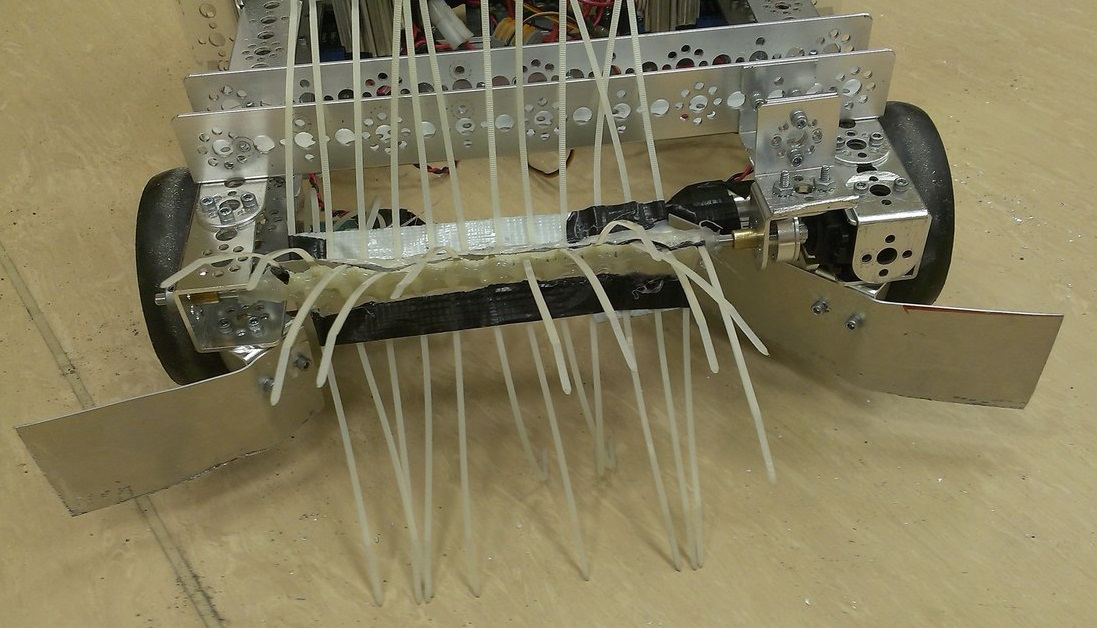
\includegraphics[scale=0.2]{days/24.10.14/images/01}}
      		\caption{Gripper with slopes}
      	\end{minipage}
      	\hfill
      	\begin{minipage}[h]{0.47\linewidth}
      		\center{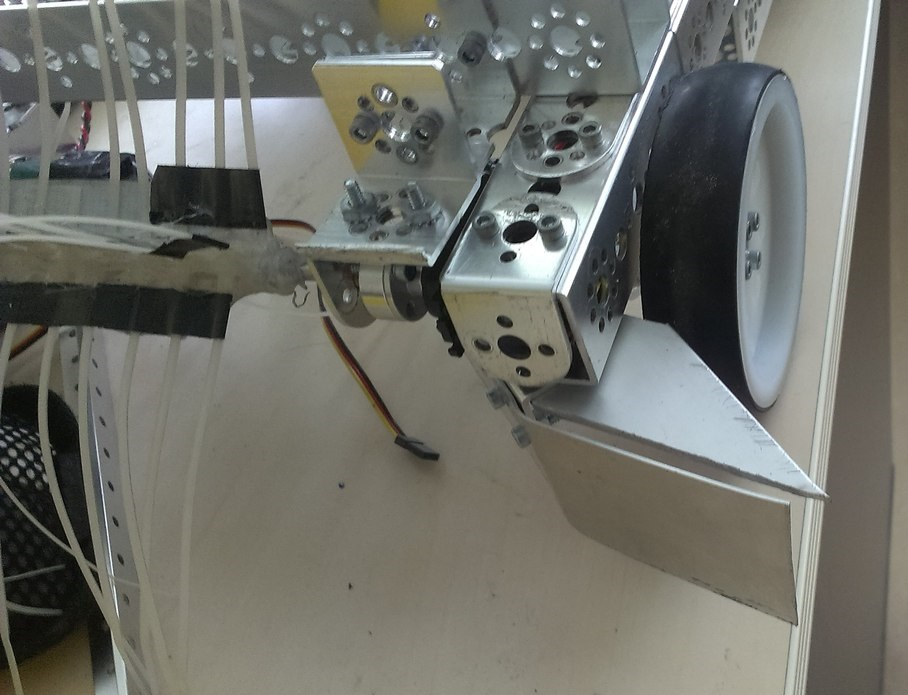
\includegraphics[scale=0.2]{days/24.10.14/images/02}}
      		\caption{Slopes with stops}
      	\end{minipage}
      \end{figure}
      
      \item The holes for installation of the remaining pair of crossbars at the lift were prepared.
      
    \end{enumerate}
    
	\item Results: 
	\begin{enumerate}
	  \item Problem with servo was corrected.
	  
      \item Slopes for balls were installed to robot.
      
    \end{enumerate}
    
	\item Tasks for the next meetings:
	\begin{enumerate}
	  \item To elaborate and create the mechanism of capture movable baskets.
	  
    \end{enumerate}     
\end{enumerate}
\fillpage
